% Drawing 148/01-10 -- folder 148, batch 01, archive page 17 (PDF page 18).
% Transcription: à gauche, première sphère, au crayon et à l'encre : l'équateur et trois méridiens issus du pôle nord ; le fuseau de gauche hachuré en rouge, celui de droite hachuré au crayon ; les pôles en rouge, des points noirs sur l'équateur, et de petits hexagones de points autour de deux sommets de l'équateur et d'un point du méridien central.
% Kind: sphere with equator and meridians, one lune hatched in red. Method 2 (schematic redraw from the facsimile). Status: partial.
% Notes: Colour render of p. 17. Pencil outline; north and south poles as red points; three meridians from the north pole down to the equator: the left one in red, the middle one in red (pencil below the equator), the right one red-brown; all three continue in pencil to the south pole. The lune between the left and middle meridians is hatched in red (horizontal strokes), the one between the middle and right meridians lightly in pencil (oblique strokes). Equator: heavy red between the left vertex and the middle point, heavy black from there to the right vertex, thin beyond; its back part dashed on the left with a black dot, another black dot at the back right. Small rings of six dots (hexagons) around the left and right vertices on the equator and, dashed, around a point just right of the middle meridian inside the upper hemisphere. Still differs: the number and slope of the hatching strokes are schematic; the ring of dots in the hemisphere sits by eye; the outline is doubled on the page and drawn once. Redrawn 2026-11-12 (issue 128): to check again.
% Coordinates: 1 unit = 1 mm = 1/100 of the crop width, y downwards as on the crop (bbox in page fractions: [0.12, 0.275, 0.4, 0.44]).
% Redrawn by Claude (claude-fable-5-2), issue #128, 2026-11-12; not checked by a human; not compiled (no TeX in the session).
% Rights: reproduces part of the work -- behind RENDER_TRANSCRIPTS, never published by itself.
\documentclass[tikz,border=3pt]{standalone}
\usepackage{amsmath,amssymb}
\usetikzlibrary{patterns,arrows.meta}
\tikzset{pencil/.style={black!45}, struck/.style={black!35}, mpt/.style={circle,draw,inner sep=1.3pt}, pt/.style={circle,fill,inner sep=0.9pt}, opt/.style={circle,draw,fill=white,inner sep=1.1pt}, Rd/.style={red!75!black}, Gn/.style={green!45!black}, Br/.style={brown!70!black}}
\begin{document}
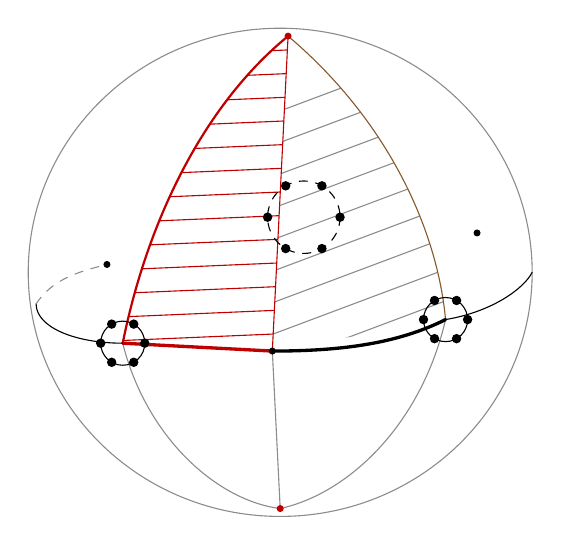
\begin{tikzpicture}[x=1mm,y=-1mm,line cap=round,line join=round,font=\small]
\coordinate (N) at (49,11);
\coordinate (S) at (48,71);
\coordinate (A) at (28,50);
\coordinate (M) at (47,51);
\coordinate (B) at (69,47);
\draw[pencil] (48,41) ellipse [x radius=32, y radius=31];
\begin{scope}
\clip (N) .. controls (38,20) and (31,35) .. (A) -- (M) -- cycle;
\foreach \y in {14,17,...,50} {
\draw[Rd,thin] (20,\y) -- (55,\y-1.5);
}
\end{scope}
\begin{scope}
\clip (N) .. controls (62,22) and (68,36) .. (B) -- (M) -- cycle;
\foreach \y in {22,26,...,66} {
\draw[pencil,thin] (44,\y) -- (76,\y-12);
}
\end{scope}
\draw[Rd,thick] (N) .. controls (38,20) and (31,35) .. (A);
\draw[Rd] (N) -- (M);
\draw[Br] (N) .. controls (62,22) and (68,36) .. (B);
\draw[pencil] (A) .. controls (31,62) and (40,70) .. (S);
\draw[pencil] (M) -- (S);
\draw[pencil] (B) .. controls (66,60) and (57,69) .. (S);
\draw[Rd,very thick] (A) -- (M);
\draw[very thick] (M) .. controls (56,51) and (63,50) .. (B);
\draw (A) .. controls (22,50) and (17,48) .. (17,45);
\draw[dashed,pencil] (17,45) .. controls (19,42) and (22,41) .. (26,40);
\draw (B) .. controls (75,46) and (79,43) .. (80,41);
\node[pt] at (26,40) {};
\node[pt] at (73,36) {};
\node[pt] at (M) {};
\node[pt,Rd] at (N) {};
\node[pt,Rd] at (S) {};
\draw (A) circle [radius=2.8];
\draw (B) circle [radius=2.8];
\draw[dashed] (51,34) circle [radius=4.6];
\foreach \a in {0,60,...,300} {
\fill[shift={(A)}] (\a:2.8) circle [radius=0.6];
\fill[shift={(B)}] (\a:2.8) circle [radius=0.6];
\fill[shift={(51,34)}] (\a:4.6) circle [radius=0.6];
}
\end{tikzpicture}
\end{document}
